\subsection{Traditional Harmony Search and some variants}
\subsubsection{Harmony Search Metaheuristic}
is a population-based metaheuristic algorithm inspired from the musical process of searching for a perfect state of Harmony or Aesthetic Quality of a Harmony (AQH). The HS was proposed by Z. W. Geem et al.\cite{DBLP:journals/simulation/GeemKL01}. In other words, the main idea of the HS metaheuristic is to mimic the process performed by musicians when they try to play a beautiful harmony.

For the purpose of properly understand what is looking like a good solution in this metaheuristic, we must know the meaning of AQH. The AQH in an instrument is essentially determined by its pitch (or frequency), sound quality, and amplitude (or loudness). The sound quality is mainly determined by the harmonic content that is in turn, determined by the waveforms or modulations of the sound signal. However, the harmonics that it can generate will largely depend on the pitch or frequency range of the particular instrument \cite{Geem:2009:MHS:1643438}. Different notes have different frequencies. For example, the note A  has a fundamental frequency $f_0=440 Hz$. The fundamental frequency of each note can be seen in (Table~\ref{fig:musical_notes}). \\		

\begin{table}[H]
\centering
\begin{tabular}{|l|l|}
\hline
\textbf{Musical Note} & \textbf{Frequency} \\ \hline
C                     & 261,625565 Hz      \\ \hline
D                     & 293,664768 Hz      \\ \hline
E                     & 329,627557 Hz      \\ \hline
F                     & 349,228231 Hz      \\ \hline
G                     & 391,995436 Hz      \\ \hline
A                     & 440,000000 Hz      \\ \hline
B                     & 493,883301 Hz      \\ \hline
\end{tabular}
\caption{HS - Musical Notes}\label{fig:musical_notes}
\end{table}

Given the above, it is established that a good harmony has good AQH. The pitch of each musical instrument determines the AQH, just as the fitness function values determines the quality of solution.

In the music improvisation process, all musicians (Table~\ref{fig:harmony_process_musician}) sound pitches (Table~\ref{fig:harmony_process_pitch_range}) within possible range together to make one harmony (Table \ref{fig:harmony_process_solution}), If all pitches make a good harmony, each musician stores in his memory that experience and possibility of making a good harmony (Table \ref{fig:harmony_process_aesthetics}) in increased next time. The same thing in optimization: the initial solution is generated randomly from decision variables within the possible range, If the objetive function values of these decision variables is good to make promising solution, then the possibility to make a good solution is increased next time.

In this document, the researcher set its focus on studying the classical SCP problem, given by equation \eqref{ec:set-covering-1}, where we want minimize the cost of solution.\\

The traditional HS metaheuristic has five steps \cite{DBLP:journals/asc/ZouGLW11}, which will be reviewed below.\\

%MUSICOS (musician - > decision variables)
\squeezeup
\begin{table}[!h]
\centering
\begin{tabular}{|m{1.5cm}|m{8cm}|}
\hline

\includegraphics[width=15mm,scale=0.05]{MarcoTeorico/imagenes/musicos.png} & 
Each musician represents a decision variable,
according to the example shown in sub-section \ref{scpSampleSolution}, there would be 11 musicians, 	
since there are 11 decision variables $x_1,\dots, x_{11}$. \\ \hline
\end{tabular}
\caption{HS components - Musician}\label{fig:harmony_process_musician}
\end{table}
\squeezeup

%--VIOLIN (Instrument Pitch Range - > Range Value of decision variable)
\squeezeup
\begin{table}[!h]
\centering
\begin{tabular}{|m{1.5cm}|m{8cm}|}
\hline
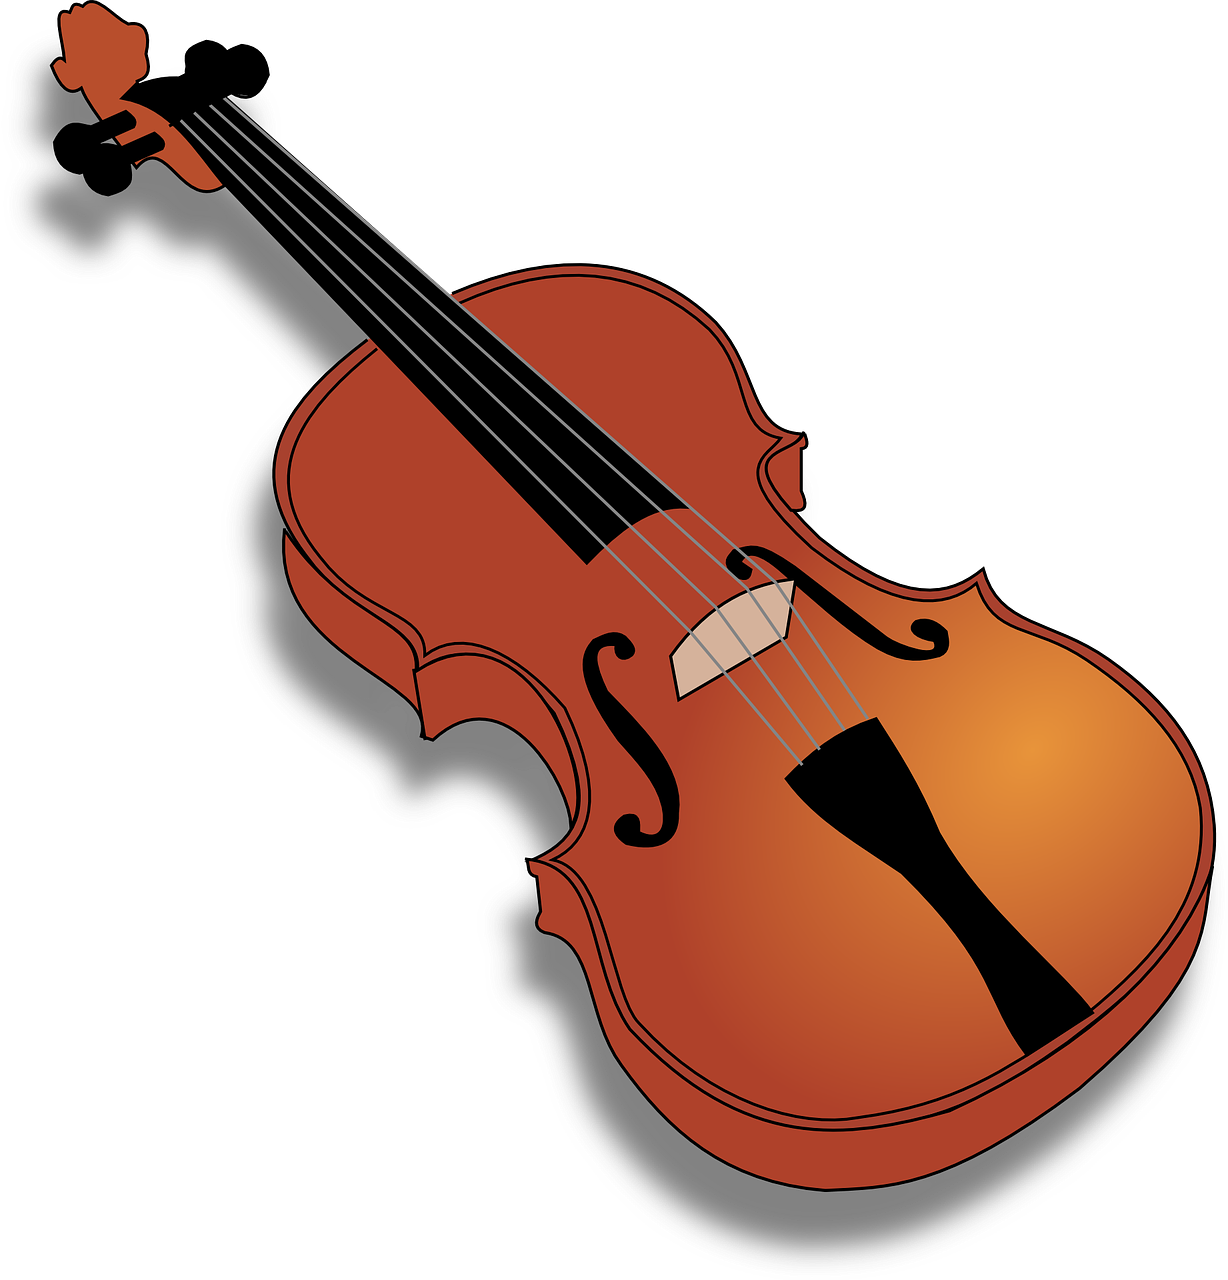
\includegraphics[width=10mm,scale=0.02]{MarcoTeorico/imagenes/violin.png} & The pitch range of the instrument represents the range of values that can take a decision variable. Given the nature of the SCP, the possible values are ${\{0,1\}}$. \\  \hline\end{tabular}
\caption{HS components - Pitch range}\label{fig:harmony_process_pitch_range}
\end{table}
\squeezeup


%--NOTA MUSICAL (Armonia -> Solucion)
\squeezeup
\begin{table}[!h]
\centering
\begin{tabular}{|m{1.5cm}|m{8cm}|}
\hline

\includegraphics[width=10mm,scale=0.0005]{MarcoTeorico/imagenes/nota.png} & Musical harmony at a certain time, corresponds to a solution at a certain iteration.\\ \hline
\end{tabular}
\caption{HS components - Solution}\label{fig:harmony_process_solution}
\end{table}
\squeezeup
% CALIDAD ESTETICA (Calidad de la armonia -> Calidad de la soluci�n)
\squeezeup
\begin{table}[!h]
\centering
\begin{tabular}{|m{1.5cm}|m{8cm}|}
\hline

\includegraphics[width=15mm,scale=0.02]{MarcoTeorico/imagenes/audience.png} & Aesthetics audience, judges whether harmony is good or not.� In the problem it refers to the objective function.\\ \hline
\end{tabular}
\caption{HS components - Aesthetics audience}\label{fig:harmony_process_aesthetics}
\end{table}
\squeezeup
%FIN TABLAS

\textbf{Step 1:  Initialize the problem and algorithm parameters.} \\
The optimization problem is defined as shown in equation \eqref{ec:set-covering-1} where the goal is to minimize $Z$ subjec to equations \eqref{ec:set-covering-2} and \eqref{ec:set-covering-3}. $x_{iL}$ and $x_{iU}$ are the lower and upper bounds for decision variables. The required parameters to solve the optimization problem, that is, Harmony Memory Size (HMS) or number of solution vectors in the harmony memory, Harmony Memory Consideration Rate (HMCR) which determines the rate of selecting the value from the memory and Pitch Adjusting Rate (PAR) which determines the probability of local improvement and number of improvisations ($NI$) are given when the metaheuristic begins.\\

\textbf{Step 2: Initialize the harmony memory.} \\
 An initial HM is filled with a population of  Harmony Memory Size (HMS). We can formally say the following: $x_i^j = x_{iL} + rand()(x_{iU} - x_{iL}), ~ j=1,2, \ldots , HMS$. Where rand() is a random from a uniform distribution of $[0,1]$.\\
 
\textbf{Step 3:  Improvise a new harmony.} \\
Harmonies are generated randomly and the details of the procedure to improvise harmony $x_i^{ \ensuremath{'}}$ can be given in Algorithm \ref{alg:impr_new_harmony}. According to the process, vectors are generated as follows $(x^1,\ldots,x^{HMS})$. Vectors results , make up a matrix such as that shown in (Figure~\ref{mat:sol_mat}):
 
 \begin{figure}
 $$
HM=
 \begin{bmatrix}
x_1^1 & \ldots & x_n^{1}\\ 
\vdots & \ddots & \vdots \\ 
x_1^{HMS} & \ldots  & x_n^{HMS}
\end{bmatrix}
$$
\caption{Harmony Memory Matrix}\label{mat:sol_mat}
\end{figure}

%ALGORITMO DE IMPROVISACION _____________________________
\squeezeup
\begin{algorithm}
      \For{$i\leftarrow 1$ \KwTo $n$}{    	
	\eIf{rand()$\leq$HMCR}
      	{
		$x_i^{ \ensuremath{'}}$ = $x_i^j$~($j=1,2,\ldots,$HMS) \mbox{//memory consideration}\\
		\lIf{rand() $\leq$ PAR} {
			$x_i^{\ensuremath{'}}$ = $x_i^{ \ensuremath{'}} \pm r(bw)$ 
      		}
      	}
      	{
        		$x_i^{ \ensuremath{'}}$ = $x_{iL}$ + rand() $(x_{iU} - x_{iL})$ \mbox{//random selection}
      	}
      }
    \caption{Generating new harmony for traditional HS}\label{alg:impr_new_harmony}
\end{algorithm}
\squeezeup
%__________________________________________________________

\textbf{Step 4: Update harmony memory.} \\
If the new generated harmony $x^{\ensuremath{'}}$ = ($x_{1}^{\ensuremath{'}}$, $x_{2}^{\ensuremath{'}}$ , \ldots,~$x_{n}^{\ensuremath{'}} $) has a better fitness than the worst one $x_{worst}$ in $HM$, then replace the worst harmony with the new one as shown in the algorithm \ref{alg:repWorstHarmony}; otherwise , go to the next step. \\

\begin{algorithm}[H]{
	%Reemplazo
	\If{fitness($x^{\ensuremath{'}}$)  > fitness($x_{worst}$)}{
   		$x_{worst} = x^{\ensuremath{'}}$\
   	}
}			
\caption{Replace worst harmony procedure}\label{alg:repWorstHarmony}
\end{algorithm}
~\

\textbf{Step 5: Check the stop criteria.} \\
If the stopping criterion (e.g. maximum number of iterations $NI$) is satisfied, computation is
terminated. Otherwise, step 3 is repeated.\\

\subsubsection{Global-Best Harmony Search Metaheuristic}
To further improve the convergence performance of HS and overcome some shortcomings of HS, a variant of HS, called  Global-Best Harmony Search (GHS), was proposed by Omran and Mahdavi \cite{DBLP:journals/amc/OmranM08}. 
The initial population in GHS is generated randomly using a Bernoulli process. Then, a greedy vector is generated $x_0$ based on a profit ratio, if $x_0$ is best than $x_{worst}$ in HM then $x_{worst}$ is replaced by $x_0$.\\
The GHS dynamically updates parameter PAR according to equation (\ref{ec:PAR-T}):

\begin{equation} \label{ec:PAR-T}
PAR(t) = PAR_{min}-\frac{PAR_{max} - PAR_{min}}{NI}t
\end{equation}

where $PAR(t)$ represents the pitch adjusting rate at generation $t$, $PAR_{min}$ and $PAR_{max}$  are the minimum and maximum adjusting rate, respectively.
The parameter $t$ is the iterative variable, and parameter $NI$ is the number of improvisations.

The parameter HMCR with a larger value can be helpful to accelerate the convergence speed, while the parameter HMCR with a smaller value can help to get out of local minima at the end of search \cite{DBLP:journals/eswa/XiangALHZ14}. The variation of the parameter depending on the iterations can be reviewed in equation (\ref{ec:MCR-T}).

\begin{equation} \label{ec:MCR-T}
HMCR(t) = HMCR_{min}-\frac{HMCR_{max} - HMCR_{min}}{NI}t
\end{equation}
~\\
where $HMCR_{min}$ and $HMCR_{max}$ represent the lower and upper bounds of $HMCR$, respectively.\\

At first, musicians most likely choose a perfect state of a harmony from their memory or harmony memory during the process of improvising a new harmony. Next, they may select a pitch from the current harmony memory randomly and then they would perform a fine tune operation, that is, pitch adjustment, for the chosen pitch to improve the effectiveness of music. For the SCP, the states of a pitch just include $\{0,1\}$, based on this, a genetic mutation is suitable for pitch adjustment \cite{286385}. The process of improvising a new harmony can be given in Algorithm \ref{alg:newHarmonyGreedy}.\\

\begin{algorithm}
\For{$j\leftarrow 1$ \KwTo $n$}{    
	\eIf{$rand(0,1) \leq HMCR(t)$}
	{
		$x_j^{ \ensuremath{'}}$ = $x_{{best}_j}$ \mbox{//memory consideration}\\
	}
	{
		\mbox{Generate a random integer number $a \in \{1,2, \dots, HMS\}$ }\\ 
		$x_j^{ \ensuremath{'}}$ = $x_{{best}_a}$ \mbox{//pitch adjustment for the pitch chosen randomly }\\
		\If{$rand(0,1) \leq PAR(t)$}{
		$x_j^{ \ensuremath{'}}$ = $\lvert x_j^{ \ensuremath{'}} - 1\rvert$	\mbox{// discrete genetic mutation }
	}
	}
	
		
}			
\caption{Generating a new harmony in GHS}\label{alg:newHarmonyGreedy}
\end{algorithm}

The Selection Mechanism is a process in which a new generated harmony vector $x_{new}$ is compared with $x_{best}$ in the first place, and if $x_{new}$ is better than  $x_{best}$, replace $x_{best}$ with $x_{new}$; otherwise  $x_{new}$ is compared with $x_{worst}$ in HM and a  greedy selection is applied between $\{x_{new}, x_{worst}\}$. As a consequence, GHS not only speeds up the convergence speed but also avoids being trapped in a local optimum. \\

\begin{algorithm}[H]{
	%Selection Mechanism
	\eIf {fitness($x_{new}$)  > fitness($x_{best}$)}{
   		$x_{best} = x_{new}$\
   	}{
		\If{fitness($x_{new}$)  > fitness($x_{worst}$)}{
   			$x_{worst} = x_{new}$\
   		}		
     	}
}			
\caption{Selection Mechanism procedure}\label{alg:SelectionMechanism}
\end{algorithm}
~\











